% 07-open: elicitation vs creation, unintended behaviours, beyond verifiable answers.

\section*{Open Problems}

\begin{frame}{Elicitation or Creation?}
  \vfill
  \centering
  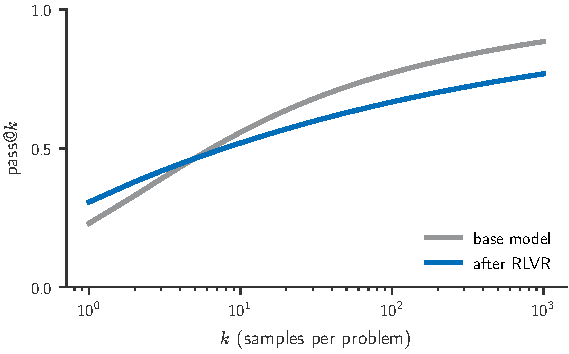
\includegraphics[width=0.85\textwidth]{s6-passk.pdf}
  \source{Schematic; shape after Yue et al., NeurIPS 2025}
  \vfill
  \keyidea{RL wins at $k=1$. At large $k$, the base model catches up.}
  \vfill
\end{frame}

\begin{frame}{Rewards That Teach the Wrong Thing}
  \vfill
  \centering
  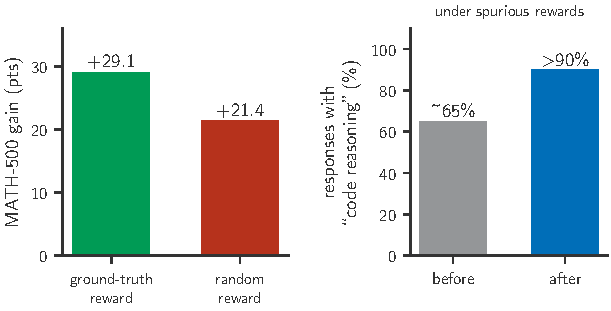
\includegraphics[width=0.85\textwidth]{s6-spurious.pdf}
  \source{Shao et al., Spurious Rewards, 2025 (Qwen2.5-Math-7B, MATH-500, GRPO)}
  \vfill
  \keyidea{Even random rewards improve accuracy. Why?}
  \vfill
\end{frame}

\begin{frame}{Beyond Verifiable Answers}
  \vfill
  \centering
  \begin{tikzpicture}
    % three equal columns of width 3.4cm on a 10.2cm bar; every row shares y
    \shade[left color=envcolor!45, right color=envcolor!5, rounded corners=3pt] (0, 0) rectangle (10.2, 0.7);
    \node[font=\footnotesize, text=black] at (5.1, 0.35) {strength of the check};
    \node[font=\LARGE\bfseries, text=black] at (9.7, 0.35) {?};
    \foreach \x/\t/\e in {1.7/{Exact check}/{Math,\\code},
                          5.1/{Partial check}/{Proofs,\\agents, QA},
                          8.5/{No check}/{Writing, advice,\\research}} {
      \node[font=\normalsize\bfseries] at (\x, 1.2) {\t};
      \node[font=\normalsize, align=center, text width=3.2cm, anchor=north] at (\x, -0.3) {\e};
    }
    \node[font=\footnotesize, text=rewardcolor, align=center, text width=3.2cm, anchor=north] at (8.5, -1.5) {rubrics? LLM judges?};
  \end{tikzpicture}
  \vfill
  \keyidea{How far does RLVR reach once the check disappears?}
  \vfill
\end{frame}
